\newpage
\section{Arquitectura física del sistema}
En la figura \ref{fig:DisenoArquiFisica} se muestra la arquitectura física del sistema, la cual abarca el diseño de la aplicación móvil así como el sistema embebido encargado de realizar las mediciones.\\

El diagrama está compuesto por dos módulos, los cuales se describen a continuación:
\begin{enumerate}
	\item \textbf{Aplicación Móvil:} Como su nombre lo indica, se refiere a la aplicación móvil, la cual es la que proporcionará el envió de notificaciones a los usuarios registrados.
	\item \textbf{Base de Datos:} Es la base de datos a la cual se comunica la aplicación móvil.
\end{enumerate}

\begin{figure}[htbp!]
	\centering
	\fbox{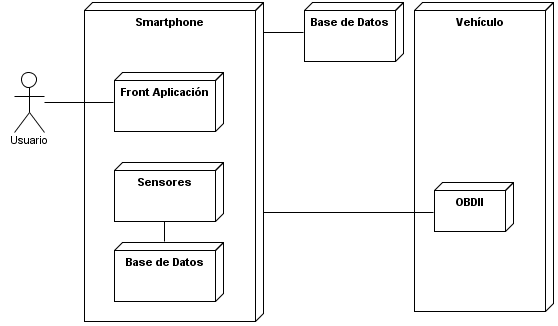
\includegraphics[width=0.9\textwidth]{DisenoEstructura/imagenes/Deployment_Diagram1}}
	\caption{Arquitectura física del sistema}
	\label{fig:DisenoArquiFisica}
\end{figure}
\clearpage

\section{Arquitectura lógica del sistema}
Una vez definidos los componentes que serán utilizados, se definió la arquitectura lógica del sistema mostrada en la figura \ref{fig:DisenoArquiLogica}, especificando la forma en que serán comunicados con el la aplicación.\\

%La figura de la arquitectura de divide en tres partes, las cuales especifican la forma de comunicación entre el sistema embebido, la red GSM y la aplicación móvil.\\

\begin{figure}[htbp!]
	\centering
	\fbox{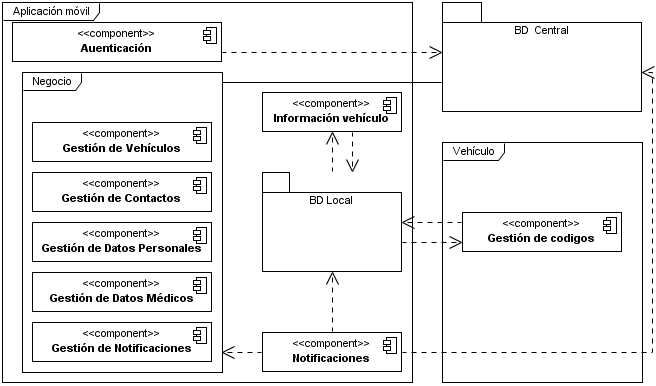
\includegraphics[width=\textwidth]{DisenoEstructura/imagenes/Arquitectura_Logica}}
	\caption{Arquitectura lógica del sistema}
	\label{fig:DisenoArquiLogica}
\end{figure}